\documentclass{scrartcl}
\usepackage[utf8]{inputenc}
\usepackage{tikz}

\begin{document}
	\title{Evaluating the ArgSearch-prototype}
	\author{Florian Euchner, Nico Weidmann and Nick Heilenkötter}
	\date{Greifswald 2018}
	\maketitle
	
	\section{Task}
	Searching the web for arguments still is a not effectively solved issue. There are some different solution approaches like \texttt{args.me}\footnote{\texttt{args.me} is the prototype implementation of the idea of searching arguments by Wachsmut et al, Bauhaus-Universität Weimar in Weimar, Germany}, but they have not been evaluated well yet. During the 2018 "Sommerakademie" in Greifswald, a scholar workshop of the German National Academic Foundation we attended the work group "Setting the news straight through technology".\\
	Our task was to implement an own search engine based on the \texttt{terrier}\footnote{text}-framework and evaluate diverse retrieval models according to relevance of the results. We did this through a assessor feedback by pooling the results.
	
	\section{The dataset}
	The dataset our search engine uses is the same as the one used by \texttt{args.me} and was provided by its creators.
	To evaluate the search engine, we needed to select some queries which results should be rated by the assessors. Therefore, we analysed the topic coverage of our dataset and  searched the \texttt{/r/ChangeMyView}-dataset to find possible relevant topics. Figure \ref{fig:common_words} shows the amount of selected  words in the titles in both datasets relative to the whole amount of words in the titles. Figure \ref{fig:common_words_arguments} shows the amount of arguments connected to these titles.
	
	\begin{figure}[hpbt]
	\centering
	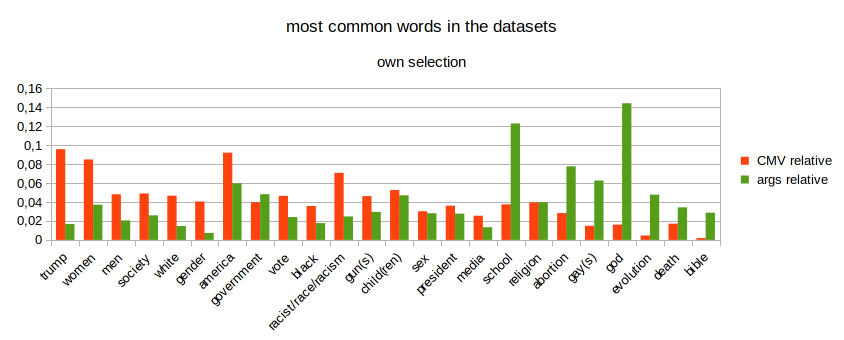
\includegraphics[height=5cm]{args_vs_cmv-words.png}
	\caption{most common words in \texttt{args.me}- and \texttt{/r/ChangeMyView}-dataset}
	\label{fig:common_words}
	\end{figure}

	\begin{figure}[hpbt]
	\centering
	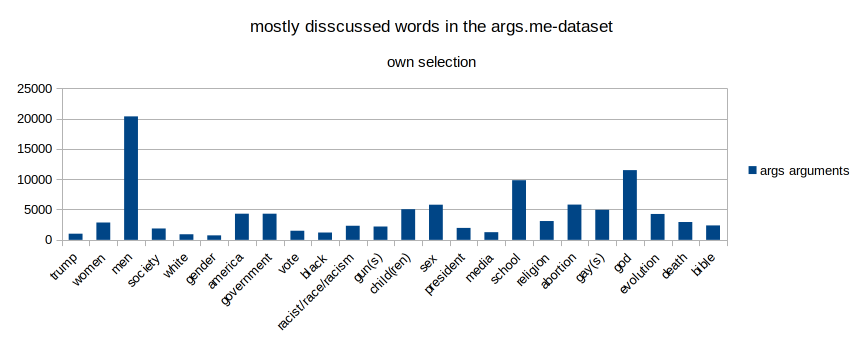
\includegraphics[height=5cm]{args_amt_of_arguments.png}
	\caption{mostly discussed topics in \texttt{args.me}-dataset achieved trough counting the number of arguments dealing with topics containing the words in figure \ref{fig:common_words}}
	\label{fig:common_words_arguments}
	\end{figure}

	\section{Evaluating the retrieval models}
	
	
\end{document}